\documentclass[aps,prb,twocolumn,groupedaddress,nofootinbib,floatfix]{revtex4}
%
\usepackage{graphicx} 
\usepackage{graphics}
\usepackage{epsfig}
\usepackage{caption}

%\setlength{\skip\footins}{0.3in}
\begin{document}
%
\title{Migration and Segregation in Three Dimensional Cellular Co-cultures: Role of
Differential Cell Adhesion and Elasticity}

%
\author{Daniel Kolbman}
%
% DON'T CHANGE ANYTHING IN THE NEXT FEW LINES OR DELETE BLANK LINES
%
\affiliation{This work was submitted as part of a course requirement for completion of the BS degree in the Physics Program at RIT and, in its current form, does not appear in any publication external to RIT.}
% % PUT YOUR ADVISOR NAME BELOW.  DON'T DELETE ANY LINES
%
\altaffiliation [Rochester Institute of Technology, School of Physics and Astronomy, Faculty Advisor: ]{Moumita Das}

\date{\today}

\begin{abstract} \noindent Mechanobiology of cell co-cultures, i.e. a binary system of cell populations, is of great interest in the biophysics of embryogenesis and tumor progression. 
During these processes, different types of cells with different physical properties are mixed with each other, with important consequences for cell-cell interaction, aggregation and migration. 
For example, the mechanics and motility of cancer cells in populations of healthy cells has been observed to be dependent on the relative stiffness of the cells. 
Until recently, experiments and theoretical models of cell co-cultures have focused on two dimensional systems.
In physiological conditions, in addition to regions of very small curvature which can be effectively assumed to be $2D$, very often cells have to navigate three dimensional micro environments.
Given that recent experiments point to very different cell migration modes in $3D$ compared to $2D$ in mono-cultures, one can ask how is cell aggregation and migration for co-culture systems different in $3D$.
To answer this question, we will model cell co-culture systems in $3D$ by extending previous $2D$ Brownian Dynamics simulation of a binary system of interacting, active and deformable particles.
Our results will be compared with ongoing experiments in the laboratory of Drs. M. Ma and M. Wu at Cornell.
These experiments are studying 3D co-cultures in confinement and in the presence of an extra cellular matrix.
Accordingly, we will study a $3D$ confined system in an underlying matrix potential.
Our results will provide insights into the role of the difference in physical properties of the two types of cells, such as stiffness and adhesion,
on emergent collective properties such as cell aggregation and migration.  

\end{abstract}

\maketitle

\section*{Background and Motivation}

Recent research provides compelling evidence for clear connections between cell mechanics and collective behavior, and the onset and progression
of several diseases including cancer. Cancer cells are cells that have undergone pathological changes, as a result of which they can divide uncontrollably, 
invade local tissue and metastasize, i.e. spread to distant parts of the body \cite{Suresh}. Metastasis is known to be the leading cause of death in cancer patients but 
its underlying physical mechanism is poorly understood. Experimental research suggests that cells  undergo dramatic changes in their physical properties such 
as cell-cell adhesion, adhesion of cells to the extra-cellular matrix, and cell stiffness during tumor progression \cite{Suresh}.
These changes may play a critical role in the enhanced aggregation and migration of cells with higher metastatic potential.
For example, for breast cancer cells the Young's modulus of the cell membrane, the cytoskeleton and the cell nucleus has 
been measured to be much smaller than that of non-cancerous breast cells \cite{Lee}.
This property has been found to affect the migration of cancer cells in the vicinity of healthy cells\cite{Lee}. 

A simple model of two dimensional homogeneous monolayers of cells  consists of interacting colloidal particles that are also each active, i.e. self-driven \cite{FilyMarchetti,RednerBaskaran}. 
Such models have been previously used to study swarming  behavior \cite{Vicsek} in birds, inspections and fish.
Our group has recently combined this approach with cell mechanics and applied it to a binary population of cells, to study the collective mechanics and dynamics in cell co-cultures characterized by a difference in cell stiffness.
Co-cultures are a valuable system to study early cancer progression, because during this process two cell populations, namely healthy cells and cells that have become cancerous may be in intermixed.   
This study found that mechanical mismatch in co-cultures can have important consequences cell migration, and can lead to enhanced motility for more deformable cells\cite{Butcher}, in agreement with
the Lee and coworkers \cite{Lee}. 

Until recently, most experiments and models of cell co-cultures have focused on two dimensional systems, with limited application to physiological conditions\cite{Jong}.
Recently, new techniques for observing co-cultures in three dimensions have become available\citep{Alessandri}.
We seek to formulate a model of cancer cell behavior in three dimensions by extending previous two dimensional simulations of binary systems of deformable and active colloids\cite{Butcher}.
Together with our experimental collaborators Drs Wu and Ma at Cornell university we aim to characterize the role of difference in physical properties -- 
cell-cell adhesion, cell stiffness and interaction with matrix, between benign and metastatic cells in cancer cell assembly and migration.
Furthermore, we will focus on confined systems to better recreate the physiological and experimental systems we are studying.
From a physics perspective, we will study the interplay of cell mechanics, and statistical mechanical in cell migration in a confined binary system in $3D$.
The main ingredients of the model are discussed below.

\begin{enumerate}

\item {\bf Co-culture Systems: mechanical stiffness and cell-cell adhesion of cancer cells vs healthy cells}\\
The co-culture environment is a vital component to the migration of cell migration \cite{Miki}.
In several biological processes from the formation of embryos to the formation of tumors, cells of different types lie and move next to each other.
In laboratory experiments, when introduced to a monolayer of healthy cells, carcinoma cells have been observed to have higher migration rates than when in a monolayer of other carcinoma cells \cite{Lee}.
In addition to the difference in stiffness \cite{Lee}, the adhesion properties of cancer cells have also been found to be drastically different from that of non-cancerous cells\cite{Jeanes}.
Most healthy cells adhere to each other via the protein E-cadherin when they come in contact, and also tend to anchor to the surrounding matrix.
Cancer cells lack this adhesiveness.
The relative adhesiveness and stiffness of the two cultures will be one of the important factors we will include in our analytical model.

\item {\bf Cell migration in three dimensions--different from $2D$ migration.}\\
Many experimental and theoretical studies have addressed various aspects of cell migration in two dimensions, including protrusion, adhesion, and retraction at the level of single cells, and collective motion at the multicellular level.
However, the {\it in vivo} environment for a crawling cell is typically a three-dimensional environment, consisting of the extracellular matrix (ECM) and surrounding cells.
Recent experiments demonstrate that cells crawling along fibers of the ECM mimic the geometry of the fibers to become long and thin, as opposed to cell migration in two dimensions where the cell is spread out in a fan shape \cite{Doyle}.
Other experiments also show increased migration rates of cells in $3D$ matrices as opposed to  $2D$\cite{Cukierman}.

\item{\bf Role of confinement}\\
Current experiments involve observing co-cultures inside of spherical capsules with diameters on the order of several hundred micro-meters and containing tens of cells\cite{Alessandri} (See FIG. \ref{fig:capsule}).
Given that confinement and finite system size can have important consequences for the statistical mechanics and collective properties of the cell-culture, it will be vital to account for them in our model.
The spherical capsules in the experiments we will model have an inner diameter of $50-700$ micro-meters and an outer diameter of $400-7000$ micro-meters.
The cells are present inside the inner capsule and have a dimensions of the order of $\sim 10$ micro-meters.
The region between the inner and outer diameters is occupied by a dense gel layer that the cells can not penetrate.
The outside of this layer is coated such that cells will not adhere to this layer. 

\begin{figure}
  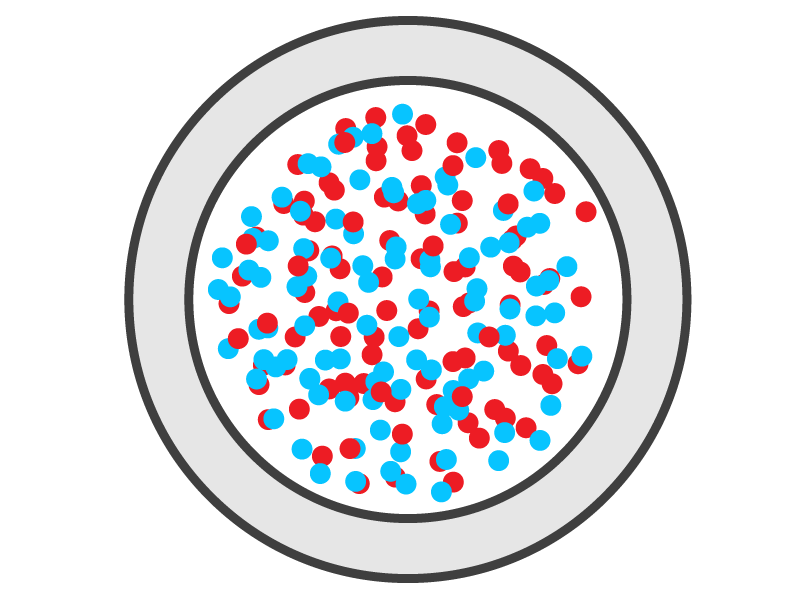
\includegraphics[width=3in]{Fig1.png}
  \caption[capsule]
   {A cross section of a spherical capsule enclosing a binary mixture of 
   cells.}
   \label{fig:capsule}
\end{figure}



\item{\bf Interaction with the extra cellular matrix}\\
The ECM is a structural network of fibers that interact with the contained 
cells \cite{Alberts}. Healthy cells adhere to the ECM and move along it in
a manner mimicking $1D$ motion. Migration of cells in this manner has been 
observed to be significantly higher than in two dimensional matrices
\cite{Doyle}. Considering the ECM and its properties will thus be very 
important in the development of our three-dimensional model.

\end{enumerate}

\section*{Model}

We will study the collective dynamics of this system using an active Brownian Dynamics simulation.
Brownian dynamics is ideal for this system
as cells behave like Brownian particles: their dimensions and times scale of motion are much larger than that of the particles of the surrounding  medium in which they are suspended and in equilibrium  their motion is diffusive.
This motion is described by the ``over-damped" Langevin equations, i.e. the inertial or acceleration term is $zero$.
In Brownian Dynamics, we study the coupled equations of motion of the Brownian particles, or in our case, cells.
The contribution of the medium particles is treated as a fluctuating force, often described in terms of a Gaussian noise.
In addition our system is ``active" because cells can generate their own forces by consuming ATP.
The overdamped Langevin equation of a representative cell is as follows\cite{Lemons}: 

\begin{equation}
F(r _m) - \gamma \frac{dr_m}{dt} + \eta(t) = 0
\end{equation}

Where $F$ is the total force on the cell and $r_m$ is its position.
This force includes contribution from cell elasticity,
cell-cell adhesion, cell-matrix adhesion and active forces.
The constant $\gamma$ is the damping coefficient of the fluid used and $\eta$ is a fluctuating force to approximate collisions with smaller particles and follows the fluctuation dissipation theorem:
\vspace{0.3in}
\begin{equation}
\left\langle \eta(t)\eta(t')\right\rangle = 0 
\end{equation}
\begin{equation}
\left\langle \eta(t)\eta(t')\right\rangle = 2k_bT\gamma
\delta(t-t')
\end{equation}

The above active overdamped Langevin equation \cite{RednerBaskaran,FilyMarchetti} has already been used in the study of binary active colloids in $2D$ \cite{Butcher}. 
We will begin by extending the $2D$ co-culture system to $3D$, then modify and add other model ingredients.

\begin{figure}
  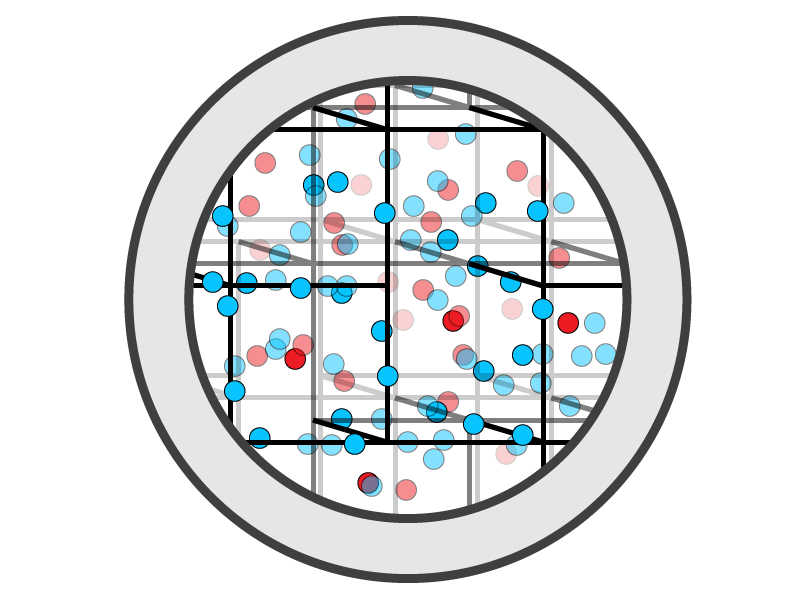
\includegraphics[width=3in]{Fig2.png}
  \caption[capsuleECM]
   {A cross section of a spherical capsule enclosing a binary mixture of 
   cells and an extracellular matrix.}
   \label{fig:capsuleECM}
\end{figure}

First, the previously used periodic boundary conditions will need to be made into spherically confined boundaries.
This will be necessary to mimic the experiments we seek to model.
We then look to incorporate co-cultures with different elastic and adhesive properties. 
Finally, we will add a qualitative extra-cellular matrix (ECM) with constant stiffness and adhesion modeled as a disordered potential (See FIG. \ref{fig:capsuleECM}). 
We will work closely with experimental results to calibrate parameters such as relative cell elasticity, diffusion constants of the cells, adhesion forces between cells and ECM, cell proportions, matrix stiffness, and system size.
Our goal is to have a model consistent with experimental set-up which will allow us to compare with experimental results.

There are further corrections that are hard to measure experimentally, but we can calculate their optimum values by using our simulations to closely imitate {\it in vivo} conditions. 
These are factors such as varying ECM density, cell-cell adhesion, and self propulsion speed of cells.
These additions will help to predict situations not yet studied experimentally and suggest areas for further development in experimental techniques. The successful accomplishment of our goals will provide
new insights for cancer cell migration in $3D$.

\section*{Budget}
\begin{itemize}\itemsep1pt \parskip0pt
\item \$100 - Textbooks, journal articles
\item \$150 - Travel
\item \$50 - Software Licenses
\end{itemize}

\section*{Goals and Timeline}

{\bf Capstone I}
\begin{itemize}\itemsep1pt \parskip0pt 
\item Brownian Dynamics for One Species Model in $3D$, with confined boundary conditions to mimic a spherical $3D$ capsule (4 weeks).
\item Extend to binary System, with different stiffness for two the two cell types. (3 weeks)
\item Add differential cell-cell adhesion for the two cell types. (3 weeks) 
\item Collect Data, Analyze Results (3 weeks)
\item Examine physical and biological implications of results, present results obtained so far 
at local conference, write paper, talk (2 weeks)
\end{itemize}
{\bf Capstone II} 
\begin{itemize}\itemsep1pt \parskip0pt
\item Apply experimental values for the inputs to the model, identify physiologically relevant regimes of parameters
and compare results of model thus far with control experiments in collaboration with Drs. Wu and Ma at Cornell. (2 weeks) 
\item Add extra cellular matrix in the form of a disordered weakly attractive potential. (4 weeks) 
\item Add self propulsion forces.(2 weeks)
\item Obtain results and analyze and interpreted  data. (2 weeks)
\item Attend March Meeting and present results (1 week)
\item Calculate phase diagram of aggregation and migration speed in terms of differential 
cell stiff, cell-cell adhesion, cell-matrix adhesion using experimentally relevant parameters. (2 weeks)
 \item Compare final results with experiments  write paper, give talk. (2 weeks)
\end{itemize}

\begin{acknowledgments}
Greatest thanks to: Dr. Moumita Das for her mentorship and assistance, Julian Butcher for his work in soft active colloids, Drs. Minglin Ma and Mingming Wu for their anticipated collaboration and experimental results, and Dr. Linda Barton for her arranging of Capstone Preparation.
\end{acknowledgments}

%
%change the name of the bibliography file to your own name
%make sure you have h-physrev5.bst file in the same directory as your tex file and bib file
%then compile using Latex-Bibtex-Latex-Latex sequence!
%

\bibliographystyle{h-physrev5.bst}
% now the actual bibliography file.   Note that it does not need the .bib extension in this line!
\bibliography{DanKolbmanBibliographyFile}
\end{document}

